\chapter{Theoretical Background}

\section{The model}

\subsection{L\'evy walks}

The original motivation for the creation of the L\'evy walk model goes back to the work of Richardson in 1926 \cite{richardson}, who studied the motion of particles in the turbulent flow of the atmosphere. Such a system contains jets and eddies that affect the behavior of the particle and lead to anomalous diffusion. In particular Richardson found that the \gls{msd} of the particle scales with the third power of the time, i.e.

\begin{align}
\mean{\ve{x}^2}(t) \propto t^3 ,
\end{align}
%
which is known as the Richardson regime.\\

There were several attempts to find a random walk model that replicates this behavior. These attempts found that power-law models were particularly suitable for describing superdiffusion \footnote{meaning diffusion where $\mean{\ve{x}^2}(t) \propto t^{1+\alpha}$, $\alpha>0$} which lead to the creation of the L\'evy flight model: In this model the walker jumps instantaneously in a random direction with a jump length drawn from a distribution $g(\abs{\ve{x}})$. He now waits at the change point for the duration of the waiting time, which is drawn from the distribution $\gls{psi}(t)$ and then performs a new jump in another direction, as can be seen in Fig. \ref{fig:levyFlight}. Both the waiting time and the jump length distributions are power-laws, meaning for large arguments they take the form 

\begin{align}
\gls{psi}(t) \propto t^{-1-\gamma}, \qquad g(\abs{\ve{x}}) \propto \abs{\ve{x}}^{-1-\beta}, \qquad \gamma, \beta > 0.
\end{align} 
%
\begin{figure}
\begin{center}
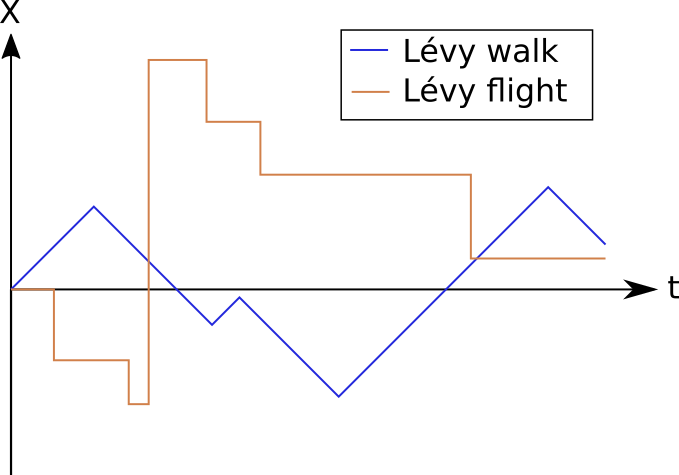
\includegraphics[width=90mm]{pics/levyFlight.png}
\caption{Comparison between the trajectories of the one dimensional L\'evy flight and L\'evy walk (for $\nu=1$). Note that the jump length of the L\'evy flight is independent of the waiting time. 
\label{fig:levyFlight}}
\end{center}
\end{figure}
%
However the L\'evy flight model has a major drawback: Since the jumps happen instantaneously it has an infinite propagation speed, which causes its \gls{msd} and all higher moments to diverge \cite{lwreview}. \\


Therefore the L\'evy walk model was developed by Shlesinger, Klafter and West \cite{shlesinger1987}. Here the walker no longer waits at the change points, but his jumps now have a finite duration, change them into steps. The step duration is coupled to the length of the step and prevents the infinite propagation speed that caused problems with the L\'evy flights, which is illustrated in Fig. \ref{fig:levyFlight}. \\

The path of a walker in the new model is now described by a series of step durations $\gls{dur}_1, \gls{dur}_2, ...$ which are drawn from the power-law distribution 

\begin{align}
\gls{psi}(\gls{dur}_i) = \frac{\gamma}{t_0} \frac{1}{(1+\gls{dur}_i/t_0)^{\gamma+1}} .
\label{eqn:defPsiT}
\end{align}
%
Here the parameter $\gamma>0$ governs the width of the distribution and { \color{red}$t_0$ is the timescale of a step }. These step durations are associated with their respective steps vectors $\ve{x}_1, \ve{x}_2, ...$, whose direction is chosen randomly. By partially summing up the step durations and the step lengths one obtains the change times $\gls{ttime}_n$ and the change points $\gls{tpoint}_n$ respectively:

\begin{align}
\gls{ttime}_n = \sum_{j=1}^n \gls{dur}_j , \qquad \gls{tpoint} = \sum_{j=1}^n \ve{x}_j
\end{align}
%
The walker is now being observed at the observation time $t$: Let the last change time before $t$ be $\gls{ttime}_n = \text{ max} \{\gls{ttime}_i | \gls{ttime}_i \leq t \}$, then the distance covered from the last change point is given by

\begin{align}
\abs{\ve{x}_{n+1}} = c (\gls{dur}_{n+1})^{\nu-1} (t-\gls{ttime}_n) ,
\end{align}
%
where c is a constant with dimension $ [ s t^{-\nu} ] $ . The speed 

\begin{align}
\gls{speed} = \pder{}{t} \abs{\ve{x}_{n+1}} = c (\gls{dur}_{n+1})^{\nu-1}
\end{align}
%
is therefore constant during the entire step but depends on the step duration $\gls{dur}_{n+1}$, where the parameter $\nu>0$ governs this dependence. \\
For any completed step we can now write down the joint probability to make a step of length $\abs{\ve{x}}$ and duration $\gls{dur}$:

\begin{align}
\gls{psi}(\ve{x}, \gls{dur} ) = \frac{\gamma}{t_0} \frac{1}{(1+\gls{dur}/t_0)^{\gamma+1}}  \frac{\delta(\abs{\ve{x}} - c \gls{dur}^{\nu}) }{\abs{\gls{step}}^{d-1} \abs{S^{d-1}}}  \label{eqn:defPsiXT}.
\end{align}
%
Here $d$ is the spatial dimension of the process and $\abs{S^{d-1}}$ is the surface area of a d-dimensional unit ball. Note that both the step duration distribution and the joint distribution are denoted by $\gls{psi}$, but their arguments are different. \\
In conclusion we have a model that is governed by two parameters, $\nu$ and $\gamma$ and can produce different kinds of anomalous diffusion.\\

Because of this versatility the L\'evy walk model is used to describe a variety of systems: Besides the application in turbulent systems for which the model was originally invented it finds application in field like biology, where  the special case of fixed velocities ($\nu=1$) is used to approximate the motion of E. coli bacteria, who move with the help of microscopic flagella. These flagella either rotate in a synchronized manner, which leads to long stretches of relatively fast movement, or unsynchronized, which leads to a tumbling motion in which the bacterium changes its direction. The resulting motion was found to follow a power-law distribution with parameter $\gamma = 1.2$ \cite{korobkova2004}

\todo{more examples: light scattering, chaotic Hamiltonian systems}



However it was found recently in \cite{radons2018} that the \gls{msd} of the model is actually divergent for certain values of its parameters, a fact that had previously gone unnoticed for the three decades of the models existence. 
The divergence can be seen directly when one writes down the contribution to the second moment of the distribution from the trajectories, that consist only of a single step longer than the observation, i.e. where the particle never stops:

\begin{align}
\mean{\ve{x}^2}(t) \geq& \int_{\mathbb{R}^d} \int_{t}^{\infty} \abs{\gls{step}}^{2}(t') \gls{psi}(\gls{step},t') dt' d^{d}x \\
=& \frac{\gamma}{t_0} \int_{0}^{\infty} \int_{t}^{\infty} \abs{\gls{step}}^{2}(t')  \frac{1}{(1+t'/t_0)^{\gamma+1}}  \delta(\abs{\gls{step}} - c (t')^{\nu-1}t)  dt' d\abs{\gls{step}} \\
=& \frac{\gamma t^2}{t_0}  \int_{t}^{\infty}   \frac{c^2 (t')^{2\nu-2}}{(1+t'/t_0)^{\gamma+1}}    dt'  .
\end{align}
%
The integrand is proportional to $(t')^{2\nu-\gamma-3}$, therefore the integral will diverge at infinity whenever $2 \nu \geq \gamma +2$ holds. This includes the parameter region where the Richardson regime was expected, so the model that was essentially invented to cure the divergence in the description of the Richardson regime turns out to be divergent itself. In order to remedy this, a more general model model is necessary.

\todo{Say something about ballistic cone?}

\subsection{Generalized L\'evy walks}

Because the divergence of the second moment is caused by very long steps that result in arbitrarily high velocities throughout the entire step, a solution can be found by letting the particle start with a lower initial speed and compensating for the slower start by accelerating it throughout the step, so that it catches up with its constant velocity counterpart at the end of the step. \\
There are indeed some models that describe particles under acceleration \cite{schulz1997, BarkaiKlafterBuch} that are similar to the Drude model for solids. There it is shown that the MSD exists in the regime where one would expect the Richardson law. \\
Furthermore in the supplementary material of \cite{radons2018} a model is presented that introduces an additional parameter, $\eta$, that allows one to interpolate between the original L\'evy model and the Drude like sheme. It is this model, which I will call generalized L\'evy walk model, that I will investigate in this thesis. \\

The generalized model uses the same distribution of step durations as the previous model (\ref{eqn:defPsiT}), but the position between two change points is calculated differently. Instead of a linear time dependence we now have a dependence on the new parameter $\eta$ for the displacement in the (n+1)th step:
%
\begin{align}
\abs{\ve{x}_{n+1}} = c (\gls{dur}_{n+1})^{\nu-\eta} (t-\gls{ttime}_n)^{\eta} .
\end{align}
%
Therefore the particle moves in general with a non-constant speed  
%
\begin{align}
\gls{speed} = c \eta (\gls{dur}_{n+1})^{\nu-\eta} (t-\gls{ttime}_n)^{\eta-1} .
\end{align}

We note, that this changes neither the change points, nor the change times and the distribution of completed steps is still given by 

\begin{align}
\gls{psi}(\ve{x}, \gls{dur} ) = \frac{\gamma}{t_0} \frac{1}{(1+\gls{dur}/t_0)^{\gamma+1}}  \frac{\delta(\abs{\ve{x}} - c \gls{dur}^{\nu}) }{\abs{\gls{step}}^{d-1} \abs{S^{d-1}}}  .
\end{align}


\begin{figure}
\begin{center}
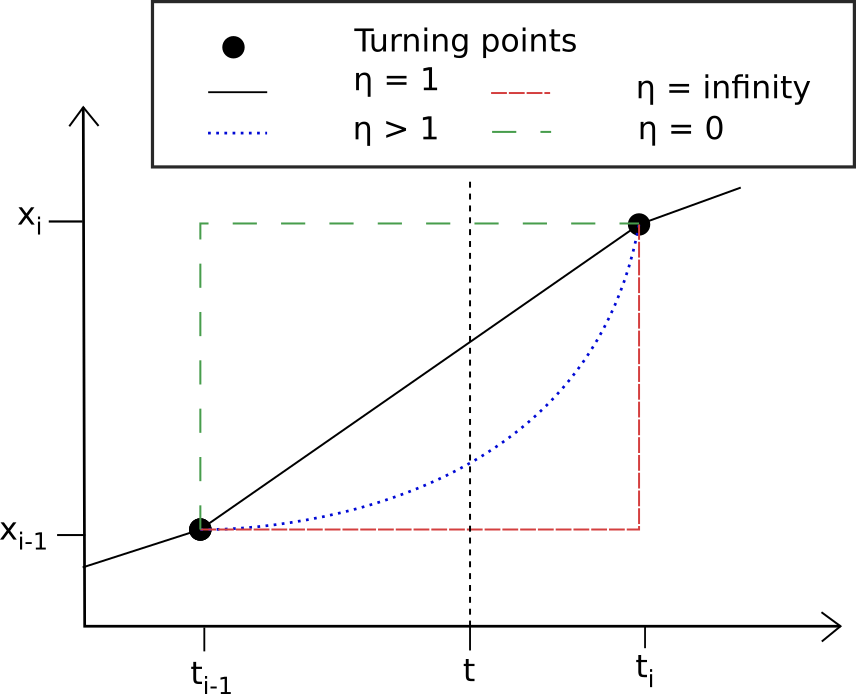
\includegraphics[width=90mm]{pics/turningPoints.png}
\caption{Comparison of the walkers motion for different values of $\eta$: The trajectories and change points remain the same, but the position measured at time $t$ varies. For $\eta = 1$ the walker moves with constant speed and has some non-linear time dependence for $\eta > 1$. In the limits $\eta = 0$ and $\eta = \infty$ we replicate the time-coupled L\'evy flight, where the two limits correspond to the walker jumping first and the then waiting or waiting first and then jumping. 
\label{fig:turningPoints}}
\end{center}
\end{figure}

However as is pointed out in the supplementary material of \cite{radons2018} the position in between two change times now depends on $\eta$, which is  illustrated in Fig. \ref{fig:turningPoints}. This affects the last incomplete steps of the walk, which we have seen to be responsible for the divergence in the original model. \\
To summarize, the generalized model now depends on three parameters: $\nu$ determines how the step length of the walker depends on the step durations, $\eta$ governs the acceleration in between the change points and $\gamma$ describes the width of the waiting time distribution. \\

{\color{blue}
To understand the reason for the anomalous nature of L\'evy walk diffusion we have to look at the moments of the steps: We can directly read off from Eq. (\ref{eqn:defPsiT}) that the mean step duration is only finite for $\gamma<1$. Furthermore we consider the distribution of lengths of completed steps, which follows from Eq. (\ref{eqn:defPsiT}) by using $\abs{\ve{x}} = c t^{\nu}$ which results in
%
\begin{align}
p(\abs{\ve{x}}) dx \propto \abs{\ve{x}}^{-\frac{\gamma+\nu}{\nu}} dx .
\end{align}
%
From this we can deduce that the mean squared step length is only finite for $2\nu < \gamma$. This is of great importance because the central limit theorem asserts that the cumulative distribution of the sum of $N$ independent identically distributed random variables of finite variance tends towards a Gaussian as $N \to \infty$. This applies to the L\'evy walk only when the mean squared step length is finite and the number of steps actually tends to infinity, i.e. when the mean step duration does not diverge. In other words, for $\gamma > 2 \nu$, $\gamma >1$ we expect the \gls{PDF} of the walk to tend towards a Gaussian in the asymptotic limit where it should show normal diffusive behavior $\mean{\ve{x}^2} \propto t$. \\
However outside these parameter ranges the walk is no longer subject to the central limit theorem. Instead it was shown by Paul L\'evy in 1920 that in this case the distribution of the sum of the variables converges to one of the so called L\'evy alpha stable distributions, which  is the statement of the generalized central limit theorem \cite{lwreview}.  

\todo{get first hand source(s) for this}
It is this close relation to L\'evy distributions that gave the L\'evy flights and later the L\'evy walks their name. The divergence of the step length is therefore not bug, but a key feature for the modeling of anomalous diffusion. \\  

A second important quality of the L\'evy walk model in general and the generalized model in particular is that it is a semi-Markov process. A process is considered Markov if the behavior of the walker after a point in time $t_0$ only depends on its position and velocity at $t_0$, not on its history. For a \gls{ctrw}, of which L\'evy walks are an example, this is usually not the case, as information about the last step, i.e. how long the walker is already moving, is important for predicting the future behavior (with the exception of Gaussian step distributions). However in our case this memory only extends to the last previous step, and the process is renewed at every change point, therefore it is semi-Markov \cite{lwreview}.\todo{first hand source} \\
Since the path of the walker is dependent on its behavior prior to the beginning of observation it is of great interest to capture this dependence through suitable initial distributions. This was investigated for similar models in \cite{barkai2003a, barkai2003b} and in this thesis the distribution of the first change point $\gls{first}(x,t|t_a)$ conditioned on the process aging for a time $t_a$ is of major importance, as it is needed to calculate the \gls{msd} of the aged walk.\\

A third related property is weak ergodicity breaking in \gls{ctrw}s. A process breaks ergodicity if its time averages and ensemble averages do not converge to the same values, usually because the trajectory of the solution observed in the time average can not reach the entire phase space, thus giving it only a partial sample. However in the case of weak ergodicity breaking the particle is able to reach the entire phase space, but the time to do this is on the same scale or larger then the total observation time, which means it does not converge reliably to the same value. \\
Ergodicity breaking is of great interest for the theoretical as well as the experimental community as it determines what results we can expect from different kinds of measurements. Power law distributions as used in L\'evy process are closely connected to weak ergodicity breaking, as their typical timescale for reaching a convergent average is divergent in subdiffusive regimes \cite{anomalousTransport}, which has been studied for example in \cite{brokmann2003,radons2018}.\\
While this thesis will not investigate the ergodicity breaking of the new model explicitly, this property is connected to the aged behavior of the walk, which is derived for the MSD. \\
}
Also note that all averages throughout the thesis are understood to be ensemble averages.
\todo{mention further generalizations of the model}
% Further generalizations of the model

\section{Theory of random walks} \label{sec:theory}
 
In this chapter I will briefly cover some of the main results of the theory of random walks that are used in this thesis. A more detailed description can be found in \cite{firstSteps}.


\subsection{Continuous time random walks}
% zoom in from RW -> CTRW -> space-time coupled CTRWs

\subsubsection{Mean number of steps}

The mean number of steps taken in a walk, $\gls{stepNumber}(t)$, gives an estimate for how fast a walker reaches the regime of asymptotic behavior that is calculated in this thesis and is therefore important for the comparison of analytical results with numerical simulations.\\
To derive a general expression for $\gls{stepNumber}(t)$ it is necessary to introduce three auxiliary quantities: The survival probability $\gls{surv}(t)$ describes the chance of a time stretch to last longer than $t$ and can be written as
%
\begin{align}
\gls{surv}(t) = \int_{t}^{\infty} \gls{psi}(t') dt' ,
\end{align}
%
where $\gls{psi}(t)$ is the distribution of time stretches. The Laplace transform of such an integral is known and results in 
%
\begin{align}
\gls{surv}(s) = \frac{1-\gls{psi}(s)}{s} \label{eqn:surv}.
\end{align}

Additionally we need the probability of starting the n-th step at time $t$, denoted by $\gls{nthStepStart}_{n}(t)$. It obeys the recursion relation
%
\begin{align}
\gls{nthStepStart}_{n}(t) = \int_{0}^{t} \psi_{n-1}(t') \gls{psi}(t-t') dt' ,
\end{align}
%
Using the convolution property of the Laplace transform (\ref{eqn:LConvolution}) and induction we find in the Laplace domain:
%
\begin{align}
\gls{nthStepStart}_n(s) = \gls{psi}^{n}(s) \label{eqn:nthStepStart}.
\end{align}

These two quantities allow us to write down the probability of being in the n-th step at time $t$, $\gls{nthStep}(t)$, i.e. the probability of having started the n-th step at time $t'$ and this step lasting longer than $t-t'$:
%
\begin{align}
\gls{nthStep}_n(t) = \int_{0}^{t} \gls{nthStepStart}_{n}(t') \gls{surv}(t-t') dt' .
\end{align}
%
Going into the Laplace domain and using results (\ref{eqn:surv}) and (\ref{eqn:nthStepStart}) we arrive at 
%
\begin{align}
\gls{nthStep}_n(s) =  \gls{nthStepStart}_{n}(s) \gls{surv}(s) = \gls{psi}^{n}(s)  \frac{1-\gls{psi}(s)}{s} .
\end{align}

The desired mean number of steps can now be expressed as the sum over the $\gls{nthStep}_n$:
%
\begin{align}
\gls{stepNumber}(t) = \sum_{n=0}^{\infty} n \gls{nthStep}_n(t) ,
\end{align}
%
which yields a closed expression in the Laplace domain:
%
\todo{see how it depends on existence of first moment}

\begin{align}
\gls{stepNumber}(s) & = \frac{1-\gls{psi}(s)}{s} \sum_{n=0}^{\infty} n \gls{psi}^{n}(s) \\
& =  \frac{\gls{psi}(s)}{s(1-\gls{psi}(s))} .
\end{align}


% introduce: survival probability, forward waiting time, step rate, mean number of steps 

% derive formula for number of steps 

% derive formula waiting times

\subsection{Space-time coupled continuous time random walks}

\todo{smooth introduction from previous chapter}

For a space-time coupled \gls{ctrw} such as the L\'evy walk a each step is determined by a joint distribution of both the step duration $\gls{dur}$ and the step distance $\gls{step}$, where the coupling between space and time is introduced by one being conditioned on the other:

\begin{align}
\gls{psi}(\gls{step}, \gls{dur}) = \gls{psi}(t) f(\gls{step}|t) .
\end{align}

We are now interested in the distribution of completed steps $\gls{comp}(x,t)$, which is the probability density that a particle starting at $\ve{x}=0$, $t=0$ reaches a change point at time $t$ and position $\ve{x}$ after an arbitrary number of steps in between. \\
A transport equation can be written down for $\gls{comp}(x,t)$ \cite{firstSteps}, which reads

\begin{align}
\gls{comp}(\ve{x},t) = \int_{-\infty}^{\infty} d^{d}\ve{x}' \int_{0}^{t} dt' \gls{comp}(\ve{x}',t')  \; \psi(\ve{x}-\ve{x}',t-t') + \delta(t) \delta(\ve{x}) . \label{eqn:CTransport}
\end{align}
%
The two terms on the right hand side express two different contributions to the probability of finding a change point at $(t,\ve{x})$: The first term is a convolution integral in $\ve{x'}$ and $t'$. It expresses the tautology that there will be a change point at $(\ve{x},t)$ exactly when there has been a change point at the primed coordinates $(\ve{x'},t')$ and the particle performed a jump with displacement $\ve{x}-\ve{x}'$ and duration $t-t'$ from $(\ve{x'},t')$ to $(\ve{x},t)$.  \\
The second term just enforces that by definition of the density we will find the particle at the origin at the beginning of observation. \\
To evaluate this integral equation it is useful to go to the Fourier Laplace domain, where the transformations are defined as follows:

The Laplace transform of a function $f(t)$ is defined as the integral 

\begin{align}
\mathcal{L} \left\{ f(t), s \right\} = f(s) = \int^{\infty}_{0} e^{-st} f(t) dt .
\end{align}
%
Note that the distinction between the function and its transform is only made in the argument of the function, which is either $t$ or $s$. \\
The Laplace transform is unique up to a set of points with Lebesgue measure zero and can be inverted via the Bromwich integral 
%
\begin{align}
\mathcal{L}^{-1} \left\{ f(s), t \right\} = f(t) = \frac{1}{2 \pi i} \int^{+i \infty + c}_{-i \infty + c} e^{st} f(s) ds, 
\end{align}
%
where $c \in \mathbb{R}$ is chosen such that $f(s)$ exists on the contour. 
\todo{move this to the first place I am using it}

For Fourier transforms I use the variables $\ve{x} \leftrightarrow \ve{k}$, with the distinction between the function and its transform being made only via the argument. It is defined as 
%
\begin{align}
\mathcal{F} \left\{ f(\ve{x}), \ve{k} \right\} = f(\ve{k}) = \int_{\mathbb{R}^{d}} e^{i\ve{k} \cdot \ve{x}} f(\ve{x}) d^{d}x ,
\end{align}
%
with inverse 
%
\begin{align}
\mathcal{F}^{-1} \left\{ f(\ve{k}), \ve{x} \right\} = f(\ve{x}) = \frac{1}{2 \pi} \int_{\mathbb{R}^{d}} e^{-i\ve{k} \cdot \ve{x}} f(\ve{k}) d^{d}k ,
\end{align}
%
where the normalization factor $\frac{1}{2 \pi}$ is kept in the inverse transform.\\

A useful property of the Fourier and the Laplace transform is that they turn convolutions of functions into simple products. In particular:
%
\begin{align}
\mathcal{L} \left\{ \int_{0}^{t} f(t') g(t-t') dt', s \right\} = f(s) g(s) , \label{eqn:LConvolution}
\end{align}
%
and 
%
\begin{align}
\mathcal{F} \left\{ \int_{\mathbb{R}^{d}} f(\ve{x}') g(\ve{x} - \ve{x}') d^{d}x' , \ve{k} \right\} = f(\ve{k}) g(\ve{k})  \label{eqn:FConvolution} .
\end{align}

Applying this to the integral equation \ref{eqn:CTransport} we obtain 

\begin{align}
\gls{comp}(\ve{k},s) =  \gls{comp}(\ve{k},s)  \; \psi(\ve{k},s) + 1 ,
\end{align}
%
and therefore 
%
\begin{align}
\gls{comp}(\ve{k},s) = \frac{1}{1 - \psi(\ve{k},s)} \label{eqn:CFourierLaplace} .
\end{align}

Our next goal is to use this result to write down an expression for the probability distribution of the ordinary, meaning non-aged, L\'evy walk $\gls{pdf}(\ve{x}|t)$. It describes the probability of finding the walker at $\ve{x}$ given that it is observed at time $t$, where it can either be at a change point or in motion, as illustrated in Fig. \ref{fig:pdfOrdinary}. 

\begin{figure}
\begin{center}
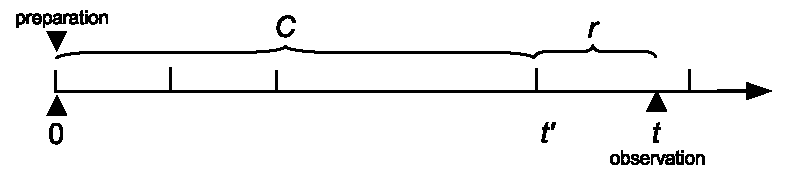
\includegraphics[width=90mm]{pics/timelineOrdinary.png}
\caption{Illustration of the path of a L\'evy walker on the time axis. Each tick on the line represents a change time. The walker starts at $t=0$ and is observed at time $t$ during a final incomplete step described by the distribution $\gls{rest}(\ve{x},t)$ after it has completed a series of steps, which is described by $\gls{comp}(\ve{x},t)$. 
\label{fig:pdfOrdinary}}
\end{center}
\end{figure}

In order to write down a transport equation for $\gls{pdf}(\ve{x}|t)$ we need to introduce the probability density for the rest of the walk after the last change point, denoted by $\gls{rest}(\ve{x}|t)$
\footnote{
Throughout the thesis I will use capital letters for probability densities that depend jointly on space and time, like $\gls{comp}(\ve{x},t)$ and lower case letters for densities that depend only on space and are conditioned on time, like $\gls{rest}(\ve{x}|t)$. Note that the former have dimension $[L^{-d} t^{-1}]$, while the latter have dimension $[L_{-d}]$.
}. 
As shown in Fig. \ref{fig:pdfOrdinary} $\gls{rest}(\ve{x}|t)$ describes the probability of the walker being displaced by the vector $\ve{x}$ after a given time $t$ during a step whose total duration is larger or equal to $t$:\\
%
{ \color{blue}
\begin{align}
\gls{rest}(\ve{x}|t) = \delta(\ve{x} - \ve{x}'(t'=t)) \int_{t}^{\infty} \gls{psi}(\ve{x}',t') dt' .
\end{align}
}
%
\\

With this expression for $\gls{rest}(\ve{x}|t)$ we can now write down $\gls{pdf}(\ve{x}|t)$ as a convolution of $\gls{rest}(\ve{x}|t)$ and $\gls{comp}(\ve{x},t)$
%
\begin{align}
\gls{pdf}(\ve{x}|t) = \int_{\mathbb{R}^{d}} \int_0^t  \gls{comp}(\ve{x}',t') \gls{rest}(\ve{x}-\ve{x}'|t-t') d t' d^{d}x' ,
\end{align}
%
which describes the particle starting at the origin, performing a series of completed steps ending at $\ve{x'}$ and then performing a final, incomplete step that leaves it at position $\ve{x}$ at observation time $t$.\\
We now use the convolution properties of the Fourier and the Laplace transform, equations (\ref{eqn:FConvolution}) and (\ref{eqn:LConvolution}), to obtain 
%
\begin{align}
\gls{pdf}(\ve{k}|s) = \gls{comp}(\ve{k},s) \gls{rest}(\ve{k}|s) \label{eqn:pdfFourierLaplaceI} .
\end{align}
%
Substituting for $\gls{comp}(\ve{k},s)$ with formula (\ref{eqn:CFourierLaplace}) yields
%
\begin{align}
\gls{pdf}(\ve{k}|s) = \frac{ \gls{rest}(\ve{k}|s)}{1 - \gls{psi}(\ve{k},s)} \label{eqn:pdfFourierLaplaceII} ,
\end{align}
%
which gives us an algebraic equation for the \gls{PDF} in the Fourier Laplace domain, that depends only on the the transforms of the step probability density and its time integral. This is a key result for the treatment of space-time coupled \gls{ctrw} {\color{blue} and will be useful for the analytical investigation into the \gls{PDF} later on.} \\

\begin{figure}
\begin{center}
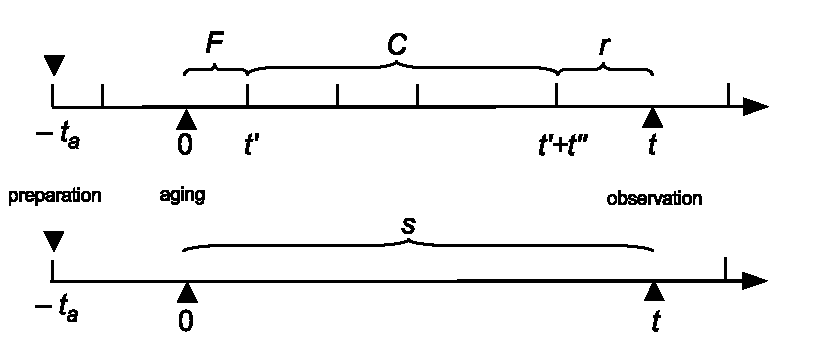
\includegraphics[width=90mm]{pics/timelineAged.png}
\caption{Illustration of an aged L\'evy walk on the time axis. Each tick on the line represents a change time. The walker starts at $-t_a$ and observation begins at $t=0$.  The upper picture shows the case where the first change time $t'$ is smaller than the observation time $t$, described by $\gls{first}$. From here it performs a series of completed steps and a final incomplete step as in the ordinary case. The lower picture shows the case that the first change point is after the end of observation, i.e. the walker never turns during observation. The probability density of this event is given by $\gls{single}$.
\label{fig:pdfAged}}
\end{center}
\end{figure}

A slightly more complicated approach is needed when aging effects are considered. In this case the walker has already moved for the duration of the aging time $t_a$ before the observation begins, which is illustrated in Fig. \ref{fig:pdfAged}. \\
At the beginning of observation, which is set to $t=0$ and $\ve{x}=0$, the walker will already be in motion and has its first observed change point some time after the beginning of observation, where we denote the probability of this change point being at $\ve{x'}$ at time $t'$ with $\gls{first}(\ve{x}',t'|t_a)$. \\
Alternatively the walker can also perform a step so long that it stays in straight motion for the entire duration of observation. In this case  no first change point is observed and this event of a long, single step is instead described by $s(\ve{x}|t,t_a)$, which is the conditional probability that a walker that has aged for $t_a$ performs a step of duration longer than $t$ such that he is at $\ve{x}$ at time $t$. \\

The transport equation for the \gls{PDF} therefore has two terms corresponding to these cases:
%
\begin{align}
\gls{pdf}(\ve{x}|t,t_a) = &\int_{\mathbb{R}^d} d^{d}x' \int_{\mathbb{R}^d} d^{d}x'' \int_{0}^{t} dt' \int_{0}^{t-t'} d t''   F(\ve{x}',t'|t_a)  \gls{comp}(\ve{x}'',t'') \gls{rest}(\ve{x}-\ve{x}'-\ve{x}''| t-t'-t'') \nonumber \\
&+ s(\ve{x}|t,t_a).
\end{align}
%
The second term captures the contribution from the single step case while the double convolution describes a particle having its first change point at $t'$, then performing a series of completed steps for the duration $t''$ and then being found at observation time $t$ in a final, incomplete step of duration $t-t'-t''$ or longer, as shown in the upper picture of Fig. \ref{fig:pdfAged}.\\
Again using the convolution property of the Fourier and the Laplace transform,  (\ref{eqn:FConvolution}) and (\ref{eqn:FConvolution}), we obtain the a closed expression for $\gls{pdf}(\ve{k}|s,t_a)$:
%
\begin{align}
\gls{pdf}(\ve{k}|s,t_a) =  \gls{first}(\ve{k},s|t_a)  \gls{comp}(\ve{k},s) \gls{rest}(\ve{k}|s) + s(\ve{k}|s,t_a) \label{eqn:pdfAgedFourierLaplace}.
\end{align}


\paragraph{Forward waiting time}

Consider a walker in a \gls{ctrw} that has aged for a time $t_a$. When the observation begins the walker will in general not be at a change point, but rather in some time interval that started before the beginning of observation. To describe this we use the forward waiting time $\gls{forwardWaiting}(t|t_a)$, which gives the probability density that the first change time after the beginning of observation is $t$ when the aging time of the walk is $t_a$. \\

In order to derive a formula for $\gls{forwardWaiting}(t|t_a)$ consider a walker starting at time zero, then performing exactly n steps that that end at $t' < t_a$ and then taking a final step of duration $t_a-t'+t$, i.e. a walker whose first change point during the observation beginning at $t_a$ is exactly at $t$. The probability density of this event is given by
%
\begin{align}
\gls{forwardWaitingNSteps}_n(t|t_a) = \int^{t_a}_{0} \gls{nthStepStart}_n(t') \gls{psi}(t_a-t'+t) dt'.
\end{align}
%
To obtain the forward waiting time we need to sum over all possible numbers of steps 
%
\begin{align}
\gls{forwardWaiting}(t|t_a) = \sum_{n=0}^{\infty} \gls{forwardWaitingNSteps}_n(t|t_a) 
= \int^{t_a}_{0} \left( \sum_{n=0}^{\infty}  \gls{nthStepStart}_n(t') \right) \gls{psi}(t_a-t'+t) dt',
\end{align}
%
which can be expressed via the step rate
%
\begin{align}
\gls{stepRate}(t) =  \sum_{n=0}^{\infty}  \gls{nthStepStart}_n(t')  \label{eqn:stepRate},
\end{align}
%
as 
%
\begin{align}
\gls{forwardWaiting}(t|t_a) = \int^{t_a}_{0} \gls{stepRate}(t') \gls{psi}(t_a-t'+t) dt'.
\end{align}

For future calculations it is useful to note that $\gls{stepRate}(t)$ has a simple form in the Laplace domain,
%
\begin{align}
\gls{stepRate}(s) = \frac{1}{1-\gls{psi}(s)} ,
\end{align}
%
which follows directly from the factorization of $\gls{nthStepStart}_n$ in (\ref{eqn:nthStepStart}).\\

In the case of a power law time distribution that lacks the first moment, e.g. the distribution for the generalized L\'evy walk (\ref{eqn:defPsiT}) with $\gamma < 1$, the forward waiting time can be calculated exactly and reads \cite{firstSteps}:
%
\begin{align}
\gls{forwardWaiting} = \frac{\sin(\pi \gamma)}{\pi} \left( \frac{t_a}{t} \right)^{\gamma} \frac{1}{t+t_a} \label{eqn:forwardWaiting} .
\end{align}

